\documentclass[tikz,border=7pt]{standalone}

\usepackage{iftex}
\ifPDFTeX
  \PackageError{matrix-figure}{This figure requires XeTeX or Tectonic}{Compile with xelatex or tectonic.}
\fi
\usepackage{fontspec}
\usepackage{xeCJK}
\usepackage{amsmath}
\usepackage{unicode-math}
\usepackage{xcolor}
\usepackage{tikz}
\usetikzlibrary{arrows.meta,positioning}

\providecommand{\FigureUseLocalFonts}{0}
\ifnum\FigureUseLocalFonts=1
  \setmainfont{NotoSansCJKtc-Regular.otf}[Path=\FigureSansFontPath]
  \setsansfont{NotoSansCJKtc-Regular.otf}[Path=\FigureSansFontPath,BoldFont=NotoSansCJKtc-Bold.otf]
  \setCJKmainfont{NotoSansCJKtc-Regular.otf}[Path=\FigureSansFontPath]
  \setCJKsansfont{NotoSansCJKtc-Regular.otf}[Path=\FigureSansFontPath,BoldFont=NotoSansCJKtc-Bold.otf]
  \setmathfont{STIXTwoMath.otf}[Path=\FigureMathFontPath]
\else
  \setmainfont{Noto Sans CJK TC}
  \setsansfont{Noto Sans CJK TC}
  \setCJKmainfont{Noto Sans CJK TC}
  \setCJKsansfont{Noto Sans CJK TC}
  \setmathfont{STIX Two Math}
\fi

\definecolor{FigureInk}{HTML}{253142}
\definecolor{RowShade}{gray}{0.84}
\definecolor{ColumnShade}{gray}{0.72}
\definecolor{ResultShade}{gray}{0.56}
\definecolor{PanelFill}{gray}{0.96}

\newcommand{\MatrixCell}[2]{%
  \tikz[baseline=(value.base)]{\node[fill=#1,rounded corners=0.4pt,inner sep=2.2pt,
    minimum width=1.35em,minimum height=1.35em] (value) {$#2$};}%
}
\newcommand{\RowCell}[1]{\MatrixCell{RowShade}{#1}}
\newcommand{\ColumnCell}[1]{\MatrixCell{ColumnShade}{#1}}
\newcommand{\ResultCell}[1]{\MatrixCell{ResultShade}{#1}}

\begin{document}
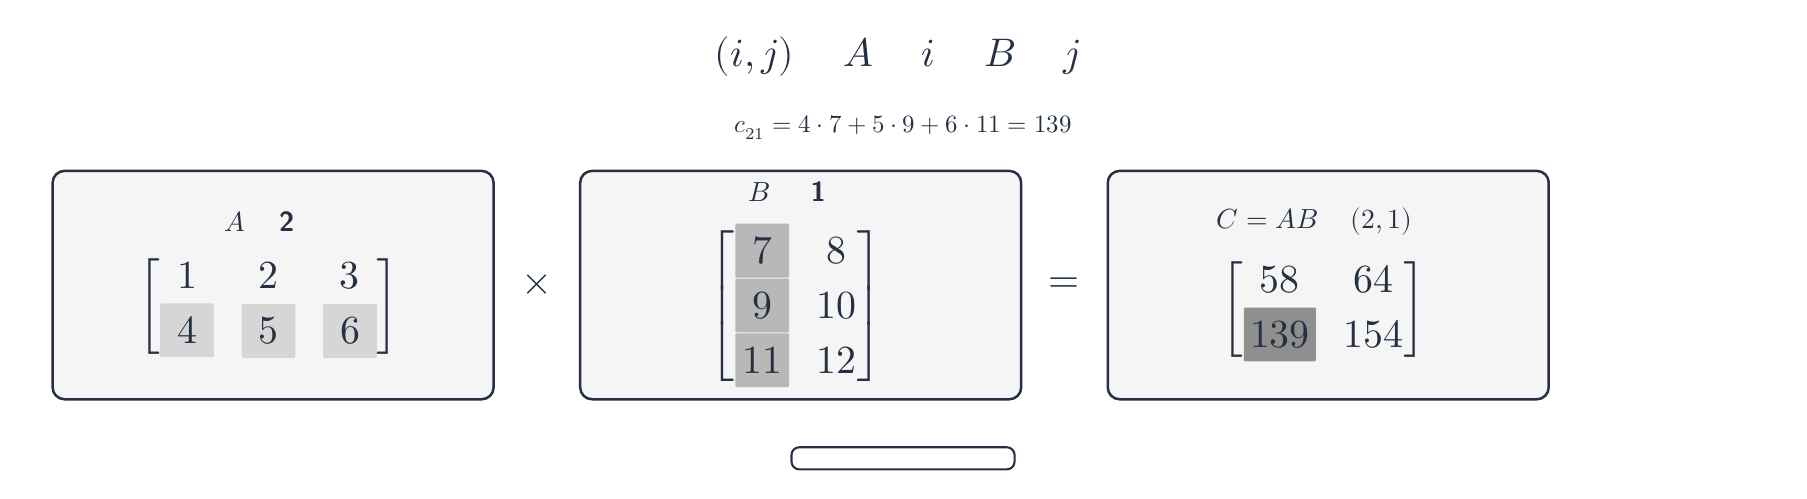
\begin{tikzpicture}[
  font=\sffamily,
  text=FigureInk,
  panel/.style={draw=FigureInk,line width=0.9pt,rounded corners=1.5mm,fill=PanelFill,
                minimum height=2.9cm,align=center},
]
  \node[font=\bfseries\Large,align=center,text width=22cm] at (11,5.65)
    {乘積的第 $(i,j)$ 元由 $A$ 的第 $i$ 列與 $B$ 的第 $j$ 行配對加總};
  \node[font=\small,align=center] at (11,4.75)
    {$c_{21}=4\cdot7+5\cdot9+6\cdot11=139$};

  \node[panel,minimum width=5.6cm] (A) at (3.0,2.75) {%
    \begin{minipage}{5.0cm}\centering
      \textbf{$A$：取第 2 列}\\[7pt]
      \Large$\begin{bmatrix}
        1&2&3\\
        \RowCell{4}&\RowCell{5}&\RowCell{6}
      \end{bmatrix}$
    \end{minipage}
  };
  \node[font=\Large] at (6.35,2.75) {$\times$};
  \node[panel,minimum width=5.6cm] (B) at (9.70,2.75) {%
    \begin{minipage}{5.0cm}\centering
      \textbf{$B$：配對第 1 行}\\[7pt]
      \Large$\begin{bmatrix}
        \ColumnCell{7}&8\\
        \ColumnCell{9}&10\\
        \ColumnCell{11}&12
      \end{bmatrix}$
    \end{minipage}
  };
  \node[font=\Large] at (13.05,2.75) {$=$};
  \node[panel,minimum width=5.6cm] (C) at (16.40,2.75) {%
    \begin{minipage}{5.0cm}\centering
      \textbf{$C=AB$：得到 $(2,1)$ 元}\\[7pt]
      \Large$\begin{bmatrix}
        58&64\\
        \ResultCell{139}&154
      \end{bmatrix}$
    \end{minipage}
  };

  \node[draw=FigureInk,line width=0.75pt,rounded corners=1mm,fill=white,
        font=\scriptsize,inner xsep=7pt,inner ysep=4pt] at (11,0.55)
    {淺灰列與中灰行的三組位置共享同一索引；深灰儲存格保存三項乘積的總和。};
\end{tikzpicture}
\end{document}
